\lstinputlisting[language=bash,basicstyle=\small]{python_codes/fieldstone_37/keywords}

\begin{center}
Code at \url{https://github.com/cedrict/fieldstone/tree/master/python_codes/fieldstone_37}
\end{center}

\par\noindent\rule{\textwidth}{0.4pt}

%%%%%%%%%%%%%%%%%%%%%%%%%%%%%%%%%%%%%%%%%%%%%%%%%%%%%%%%%%%%%%%%%%%%%%%%%%%%%%%%%%%%%%%%%%%%%%%%%%%%

The domain is a unit square. The Stokes equations are not solved, the velocity is prescribed 
everywhere in the domain as follows:
\begin{eqnarray}
u(x,y)&=&-(y-0.5)\nn\\
v(x,y)&=&(x-0.5) \nn
\end{eqnarray}

\begin{center}
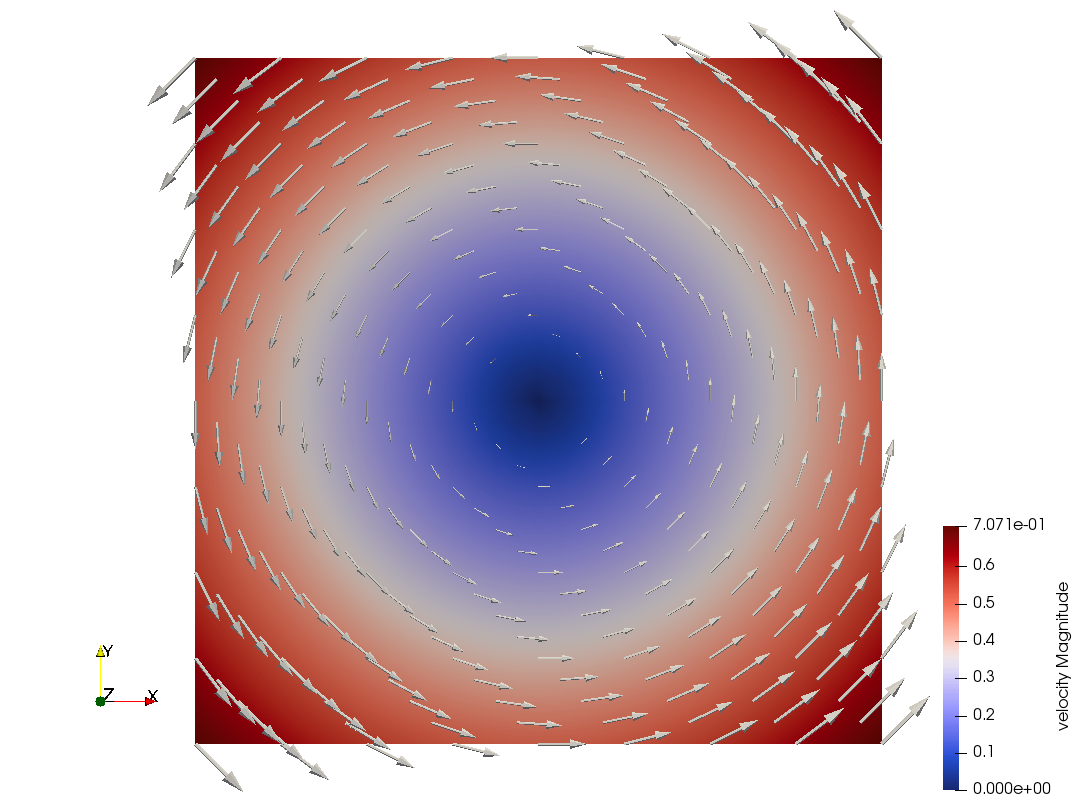
\includegraphics[width=5cm]{python_codes/fieldstone_37/vel}
\end{center}

If {\tt RKorder} is zero, then velocity is computed on the particle itself via the equation above. 
If {\tt RKorder} is 1,2,3,4,5 then the corresponding Runge-Kutta algorithm (in space) is used and basis functions are
used to interpolate the velocity from the nodes onto the particles.. 
Particles can be placed on a regular grid or randomly inside each element at the beginning.
The timestep is controlled via a CFL condition.    
When particles are advected outside the domain, they are arbitrarily placed at location (-0.0123,-0.0123).

\begin{center}
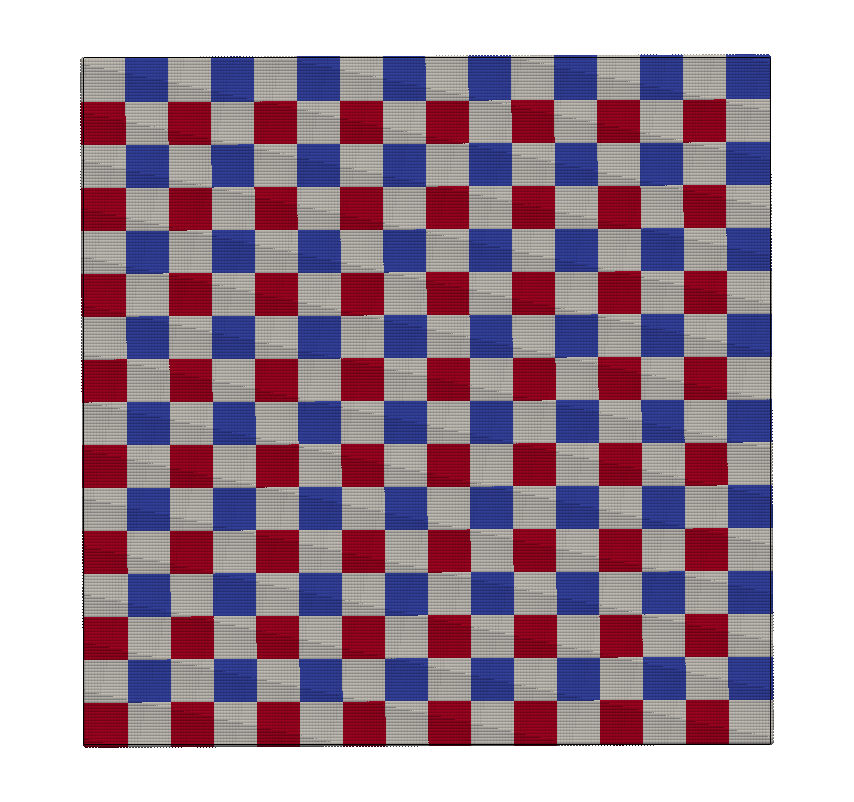
\includegraphics[width=3cm]{python_codes/fieldstone_37/particles0000}
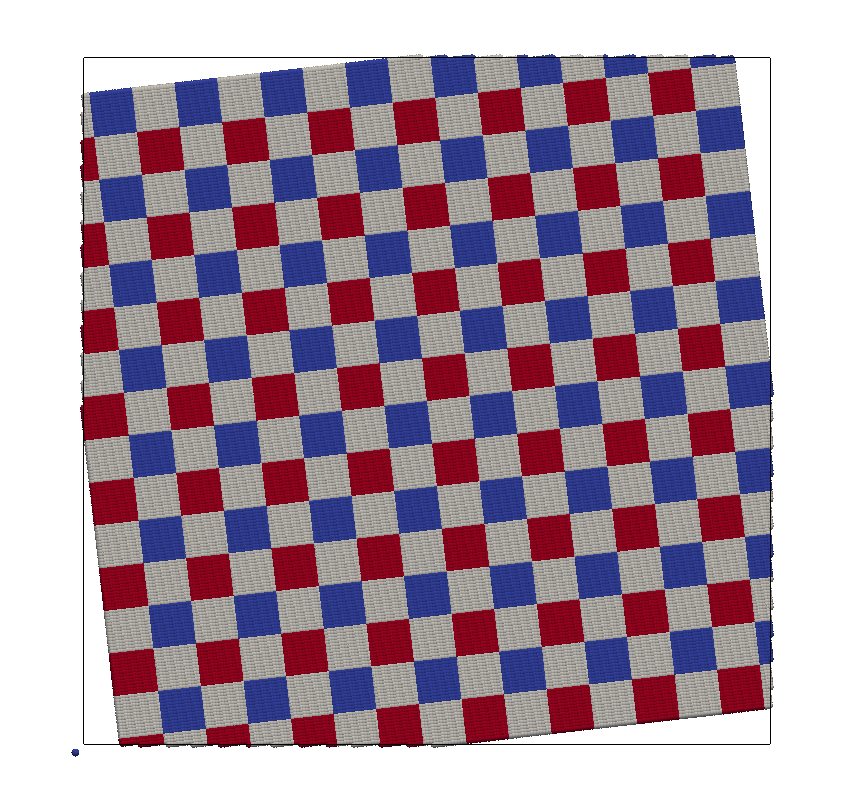
\includegraphics[width=3cm]{python_codes/fieldstone_37/particles0005}
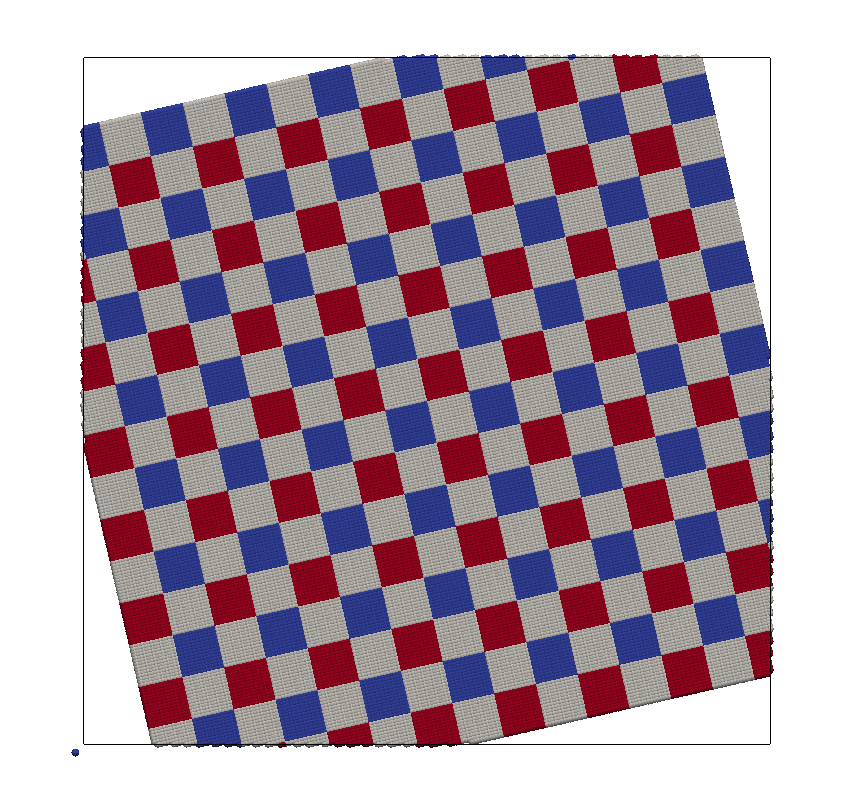
\includegraphics[width=3cm]{python_codes/fieldstone_37/particles0010}
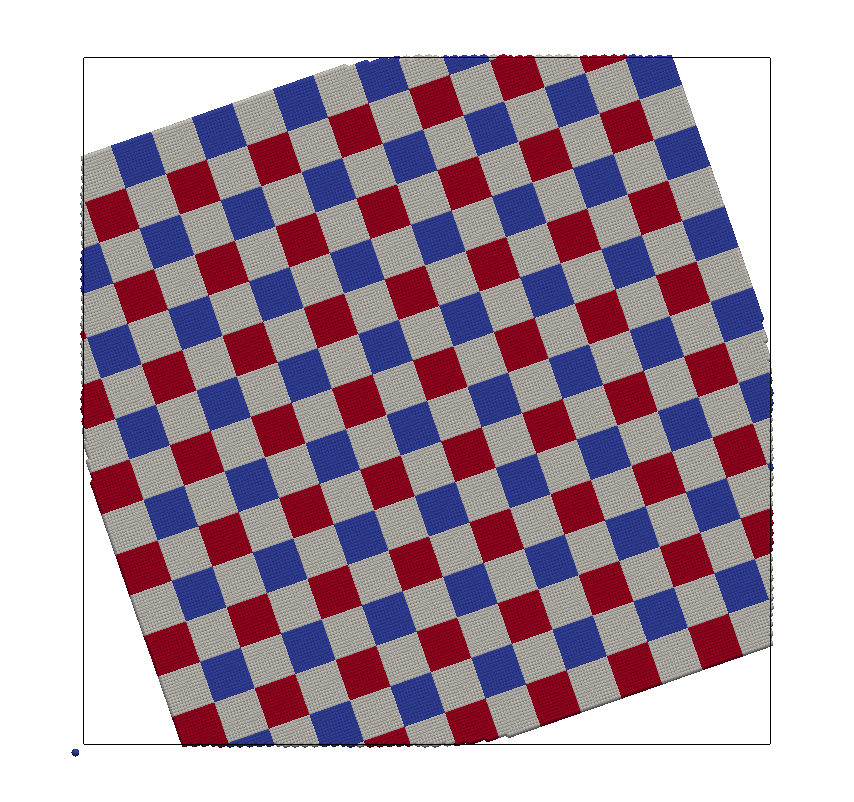
\includegraphics[width=3cm]{python_codes/fieldstone_37/particles0015}
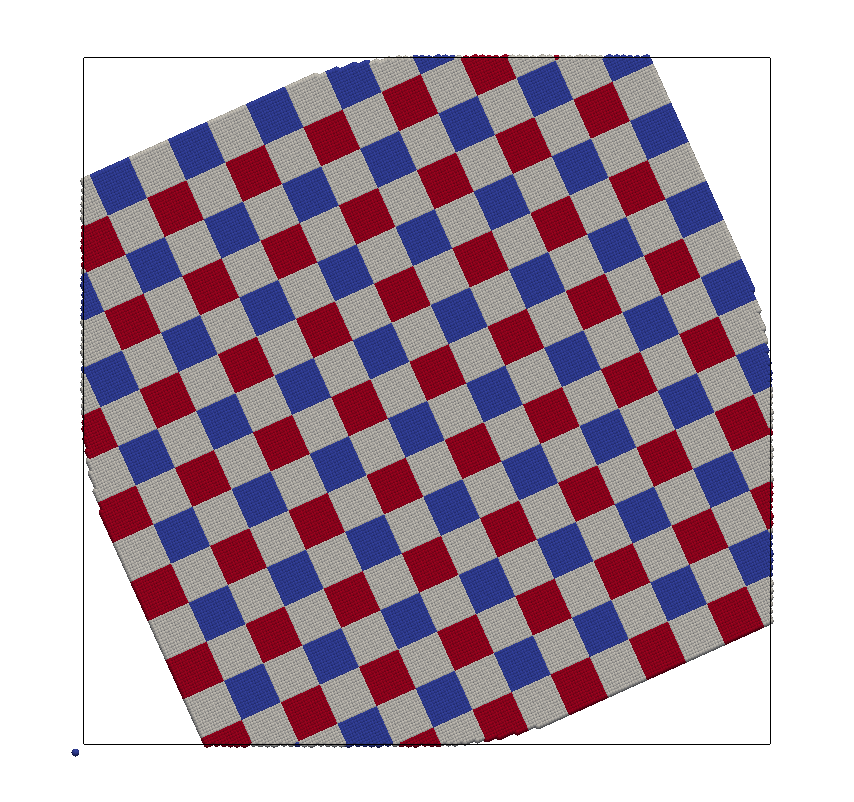
\includegraphics[width=3cm]{python_codes/fieldstone_37/particles0019}\\
{\captionfont Example with 32x32 $Q_1$ elements, $7^2$ particles, CFL=0.1, RKorder=2, regular distribution.}
\end{center}

Note that $Q_2$ elements have not been tested yet.

Also, I will some day add a population control algorithm to replenish elements with not enough particles.

